We reproduced the Japenese-to-English decipherment (i.e., without parallel data) experiments of \newcite{RK09}, whose goal is to decode a list of 100 US senator names written in Katakana, without access to parallel data.

Specifically, \newcite{RK09} construct a phonetic-based English-to-Japanese transliteration model as a cascade of wFSTs. 
That is, their model maps an English word to its phonetic pronunciation, which is then mapped to a Japanese pronunciation and finally to a word in Katakana script.
The cascade of wFSTs at the top of Figure \ref{fig:fsts} depicts the corresponding generative story.

Essential to our discussion, is the (shaded) English-to-Japanese phoneme t-table $t_1$ which allows only 1-to-1 and 1-to-2 phoneme mappings. 
This model is used to obtain a (monotonic) alignment between an English phoneme sequence and a Japanese one. 
For example, the word "computer" has a phonetic representation as a sequence of 8 English phonemes $(k, ah, m, p, y, uw, t, er)$, while its transliteration, as a sequence of 9 Japanese phonemes $(K, O, N, P, Y, U, T, A, A)$.

Using their model, \newcite{RK09} report whole-name error rates (WNER\footnote{In WNER, a decoding is correct if both the first and last name are correctly decoded}) of 40\% with parallel data (trained over 3.3K word pairs), compared to 73\% WNER without parallel data (trained over 9.5K Japanese words only), thus demonstrating a big performance gap for alignment methods that do not use parallel data.

\begin{figure*}[t]
\begin{center}
\begin{tabular}{c}
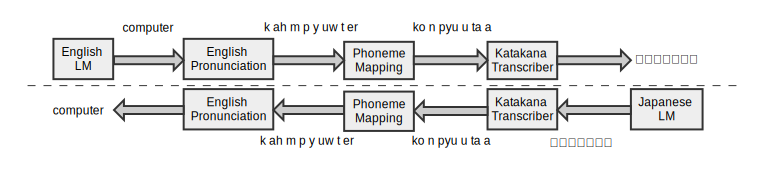
\includegraphics[scale=0.62]{figures/fsts}\tabularnewline
\end{tabular}
\caption{\label{font-table} The transliteration generative story as a cascade of wFSTs. Each box represents a transducer. \textbf{Top:} transliteration of the word ``computer'' to Japanese. \textbf{Bottom:} the reverse process. $\method{MIR}$ jointly trains the two cascades by maximizing the regularized data log-likelihood with respect to the two (shaded) phoneme mapping models. 
%The blank wFSTs are held fixed.
}
\label{fig:fsts}
\end{center}
\end{figure*}

\subsection{Forward Model}
We reproduced the English-to-Japanese transliteration pipeline of \newcite{RK09 }by constructing each wFST as follows:
\begin{enumerate}
\item A unigram language model (LM) of English terms, estimated over the top 40K most frequent capitalized words found in the Gigaword corpus (without smoothing).
\item An English pronunciation wFST from the CMU pronunciation dictionary\footnote{http://www.speech.cs.cmu.edu/cgi-bin/cmudict}.
%http://svn.code.sf.net/p/cmusphinx/code/trunk/cmudict
\item An English-to-Japanese phoneme mapping wFST that encodes a phoneme t-table $t_1$ which was designed according to the best setting reported by \newcite{RK09}. 
Specifically, $t_1$ is restricted to either 1-to-1 or 1-to-2 phoneme mappings and maintains consonant parity. See further details in their paper.
\item A hand-built Japanese pronunciation to Katakana wFST \cite{RK09}.
\end{enumerate}


%\newcite{RK09} report back-transliteration whole-name error rates (WNER) on a list of 100 transliterated US senator names (). They train the wFST cascade in both the parallel and non-parallel data settings, obtaining 40\% WNER with parallel data (trained over 3.3K word pairs), compared to 73\% WNER without parallel data (trained over 9.5K Japanese words only).

\subsection{Backward Model}
Applying $\method{MIR}$ requires a pipeline in the reverse direction -- for transliteration of Japanese to English.
We constructed a unigram LM of Katakana terms over the top 25K most frequent Katakana words found in the Japanese news 2005-2008 Leipzig corpora\footnote{http://corpora.uni-leipzig.de/}.

The remaining required wFSTs were obtained by inverting the forward model wFSTs (that is, wFSTs 2,3,4 above), and the cascade was composed in the reverse direction.
In particular, by inverting $t_1$, we obtained the Japanese-to-English t-table $t_2$ that allows only 2-to-1 or 1-to-1 phoneme mappings.

\subsection{Training Data}
For training data, we took the top 50\% most frequent terms from the constructed LM wFSTs, resulting in a set of 20K English terms (denoted $\mathtt{ENG}$) and a set of 13K Japanese terms in Katakana (denoted $\mathtt{KTKN}$).
Taking the entire set of terms in each LM led to poor baseline results, probably since uncommon English terms are not transliterated, and uncommon Katakana terms may be borrowed from languages other than English.
In any case, it is important to note that $\mathtt{ENG}$ and $\mathtt{KTKN}$ are unrelated, since both were collected over non-parallel corpora.

\subsection{Training and Tuning}

\begin{figure*}[t]
\begin{center}
\begin{tabular}{cc}
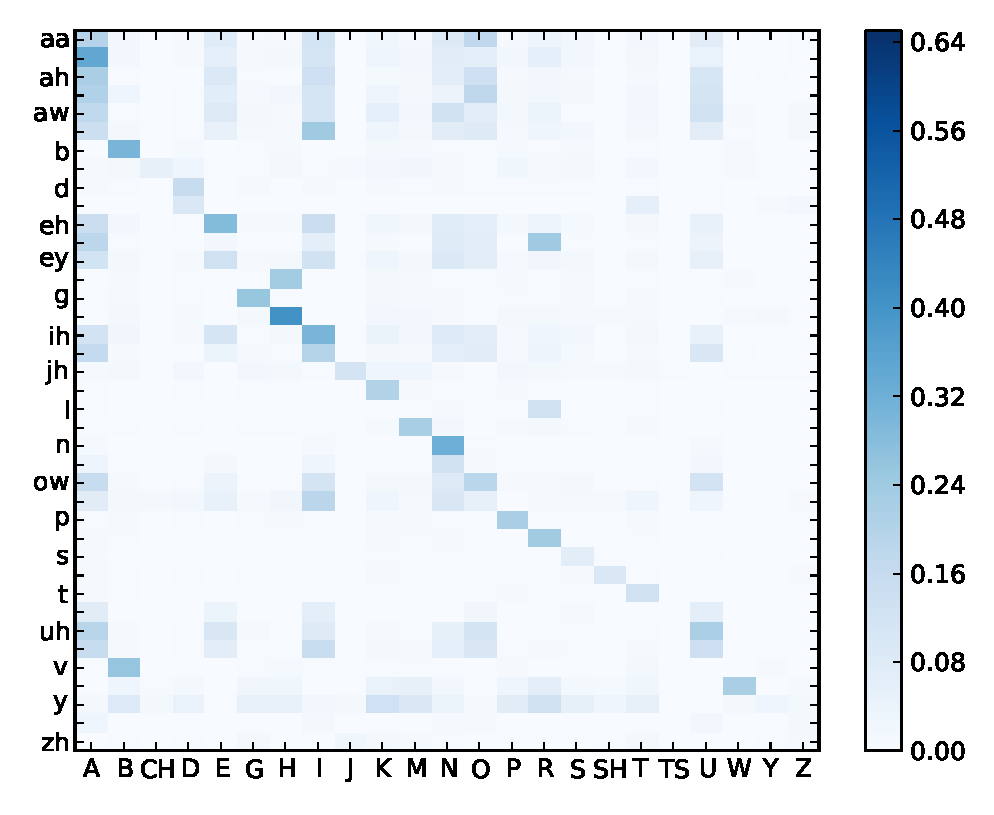
\includegraphics[scale=0.4]{figures/model_11_vanilla} & \includegraphics[scale=0.4]{figures/model_11_gm}
\end{tabular}
\caption{The 1-to-1 mapping submatrix of the $t_1$ transliteration table for independent training (left) and $\method{MIR}$ (right). $\method{MIR}$ learns sparser, peaked models than independent training does.}
\label{fig:mapping}
\end{center}
\end{figure*}

% We used the 
%This was done by manipulating Carmel to output the E-step posteriors which were then used to construct the M-step objective externally. The M-step was solved using our own PGD implementation.
We trained and tuned 4 models:
\begin{description}
\item $\method{baseline}$: the model proposed by \newcite{RK09} - maximizing the likelihood (\eqn{eqn:decipherment}) of the observed Japanese terms $\mathtt{KTKN}$.

\item $\method{MIR}$: Our bidirectional, regularized model -  maximizing the regularized likelihoods (\eqn{eqn:joint}) of both monolingual corpora $\mathtt{ENG, KTKN}$.

\item $\method{bi\mbox{-}EM}$: The joint model proposed by \newcite{Mylonakis2007} - maximizing the likelihoods (\eqn{eqn:biEM}) of both monolingual corpora $\mathtt{ENG, KTKN}$.

\item $\method{Oracle}$: As an upper bound, we trained the model of \newcite{RK09} over 4.2K \emph{parallel} English-Japanese phoneme sequences. 
\end{description} 

While training, the language and pronunciation wFSTs were held fixed, and, 
each phoneme mapping model was trained for 15 EM iteration, maximizing its respective objective. 
To train these models, we used the Carmel finite-state toolkit\footnote{http://www.isi.edu/licensed-sw/carmel/}.
Specifically, the $\method{baseline}$ and $\method{oracle}$ methods rely on Carmel exclusively, while for $\method{MIR}$ and $\method{bi-EM}$, we manipulated Carmel to output the E-step posteriors, which we then used to formulate and solve the M-step objective using our own implementation.

We tuned the different models over a development set consisting of 50 frequent Japanese terms and their English origin.
For each method, we selected the model that minimized the development back-transliteration error rate over the 15 iterations, the so-called stretch-factor 
$\alpha \in \set{1,2,3}$ used to exponentiated the model parameters before decoding (see \newcite{RK09}) and our model's $\lambda\in \set{1,2,3,4}$.

Decoding of Japanese terms was done using the Viterbi algorithm, applied on the selected $t_1$ model (We use \eqn{eqn:reparam} to convert the $\method{bi\mbox{-}EM}$ model $\theta$ to $tA$).
Note that symmetrization heuristics are not applicable since they require parallel data.


\subsection{Senator Name Decoding}
We compiled our own test set, consisting of 100 US senator names (first and last) and compared the performance of the four algorithms.

%Table \ref{tbl:transliteration0}  % ref not working for some reason
Table 2
reports WNER, average normalized edit distance (NED) and the number of model parameters with value greater than 0.01 ($t_1>0.01$) as an indication of sparsity. 
Figure \ref{fig:mapping} further compares a portion of the best phoneme mapping table learned by the baseline vs. that learned by $\method{MIR}$, depicting the difference in parameter sparsity.
\begin{table}[h]
\begin{center}
\begin{tabular}{l|c|c|c}
\multicolumn{1}{c|}{} & WNER & NED & $t_1> 0.01$\tabularnewline
\hline 
Independent & 67\% & 23.2 & 649\tabularnewline
$\method{bi\mbox{-}EM}$ & 66\% & 21.8 & 600\tabularnewline
$\method{MIR}$ & \textbf{59}\% & \textbf{17.3} & \textbf{421}\tabularnewline
\hdashline
Parallel Data & 43\% & 10.8 & 152\tabularnewline
\end{tabular}
\caption{$\method{MIR}$ reduces error rates (WNER, NED) and learns sparser models (number of $t_1$ parameters greater than 0.01).}
\end{center}
\label{tbl:transliteration0}
\end{table}

Using $\method{MIR}$ we obtained a significantly reduction in error rate, closing the gap between the baseline method and one trained on parallel-data settings by 33\% in WNER and nearly half in NED.
This error reduction clearly demonstrates the efficacy in proper joint training of these alignment models, and of the $\method{MIR}$ formulation in particular.

%
%In this section we present our experiments on deciphering transliterations.
%We first reproduced the English-to-Japanese transliteration pipeline of \newcite{RK09} (as described in Section \ref{sec:background} and depicted at the top of Figure \ref{fig:fsts}) and tried to match their reported results\footnote{Unfortunately, we were unable to obtain all their wFSTs and data.}.
%We then constructed the reverse Japanese-to-English pipeline, required for PAT, and compared the two approaches.
%
%\subsection{Baseline Decipherment Model}
%To reproduce the English-to-Japanese pipeline, we constructed the following wFST models:
%\begin{enumerate}
%\item A unigram language model (LM) of English terms, estimated over the top 40K most frequent capitalized words found in the Gigaword corpus (without smoothing).
%\item An English pronunciation wFST from the CMU pronunciation dictionary\footnote{http://www.speech.cs.cmu.edu/cgi-bin/cmudict}. %(REFERENCE?).
%%http://svn.code.sf.net/p/cmusphinx/code/trunk/cmudict
%\item A English-to-Japanese phoneme mapping wFST that encodes the phoneme transliteration table $t_1$ (see \eqn{eqn:trans}), constructed based on the best setting reported by \newcite{RK09}. 
%We note that $t_1$ is restricted to either 1-to-1 or 1-to-2 phoneme mappings, maintaining consonant parity. See further details in their paper.
%\item A hand-built Japanese pronunciation to Katakana wFST \cite{RK09}.
%\end{enumerate}
%
%\newcite{RK09} report back-transliteration whole-name error rates (WNER) on a list of 100 transliterated US senator names (In WNER, a decoding is correct if both the first and last name are correctly decoded).
%They train the wFST cascade in both the parallel and non-parallel data settings, obtaining 40\% WNER with parallel data (trained over 3.3K word pairs), compared to 73\% WNER without parallel data (trained over 9.5K Japanese words only).
%
%\subsection{Inverse Model}
%PAT requires a pipeline in the reverse direction, for transliteration of Japanese to English.
%% - a Japanese-to-English transliteration pipeline with similar FST models.
%We constructed a unigram LM of Katakana terms over the top 25K most frequent Katakana words found in the Japanese news 2005-2008 Leipzig corpora\footnote{http://corpora.uni-leipzig.de/}.
%% (REFERENCE).
%%(http://corpora.informatik.uni-leipzig.de/download.html)
%
%The remaining required wFSTs were obtained by inverting the baseline wFSTs (that is, wFSTs 2,3,4), and the cascade was composed accordingly (depicted at the bottom of Figure \ref{fig:fsts}).
%In particular, by inverting $t_1$, we obtained a Japanese-to-English wFST $t_2$ that allows only 2-to-1 or 1-to-1 phoneme mappings.
%
%\subsection{Training and Decoding}
%For training data, we took the top 50\% most frequent terms from each LM, resulting in a set of 20K English terms and a set of 22.5K Japanese terms.
%Using the whole set of terms led to poor baseline results, probably since uncommon English terms are not transliterated, and uncommon Katakana terms may be borrowed from languages other than English.
%In any case, it is important to note that the two resulting sets of words are far from being parallel, since they were collected over non-parallel corpora.
%
%Vanilla EM training of the baseline was done using the Carmel finite-state toolkit\footnote{http://www.isi.edu/licensed-sw/carmel/}. The LM and pronunciation models were held fixed while the parameters of the phoneme mapping model $t_1$ were optimized to maximize the likelihood of the observed set of Japanese terms.
%
%The $\method{MIR}$ objective (\eqn{eqn:joint}) was maximized with respect to the phoneme mapping models $(\TA, \TB) = (t_1, t_2)$, with coefficient $\lambda\in\{1,2,3,4\}$.
%We manipulated Carmel to compute a single E-step and output the posteriors which we then used to formulate the M-step objective. 
%The M-step was solved using our own PGD implementation\footnote{A general purpose PGD solver for convex functions over convex closed sets, and will be released as open-source software.}.
%
%To compare against the ordinary parallel data setting, we trained the English-to-Japanese phoneme mapping model $t_1$ with Carmel. We used 4.2K pairs of English and Japanese phoneme sequences. For all models, training was limited to 15 EM iterations.
%
%Finally, back-transliterations of Japanese terms were computed using regular Viterbi decoding of the term with the $t_1$ model only.
%Note that symmetrization heuristics are not applicable since we have no parallel data.
%
%\subsection{Results}
%\begin{figure*}[t]
%\begin{center}
%\begin{tabular}{cc}
%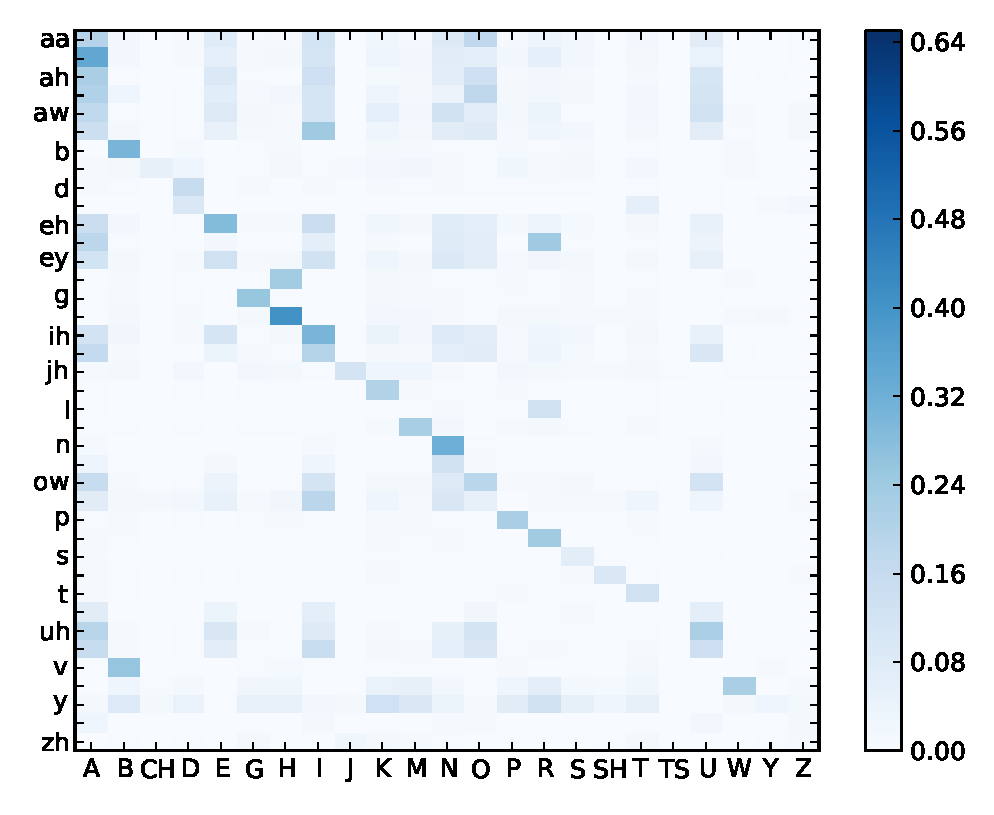
\includegraphics[scale=0.4]{figures/model_11_vanilla} & \includegraphics[scale=0.4]{figures/model_11_gm}
%\end{tabular}
%\caption{The 1-to-1 mapping submatrix of the $t_1$ transliteration table for independent training (left) and $\method{MIR}$ (right). $\method{MIR}$ learns sparser, peaked models than independent training does.}
%\label{fig:mapping}
%\end{center}
%\end{figure*}
%We compiled our own list of 100 US senator names (first and last) to be used as a test set. 
%To tune $\lambda$ we used a development set consisting of 50 frequent Japanese terms and their English origin.
%
%For each method, we selected the $t_1$ model that minimized the development back-transliteration error rate over the 15 iterations, $\lambda$ and the so-called stretch-factor 
%$\alpha \in \{1,2,3\}$ that exponentiated the model parameters before decoding (see \newcite{RK09}).
%
%%Table \ref{tbl:transliteration}  %% ref not working for some reason
%Table 1
%reports WNER, average normalized edit distance (NED) and the number of $t_1$ parameters with value greater than 0.01 ($t_1>0.01$) as an indication of model sparsity. 
%Figure \ref{fig:mapping} further compares a portion of the best phoneme mapping table learned by the baseline vs. that learned by PAT, depicting the difference in parameter sparsity.
%
%\begin{table}[h]
%\begin{center}
%\begin{tabular}{l|c|c|c}
%\multicolumn{1}{c|}{} & WNER & NED & $t_1> 0.01$\tabularnewline
%\hline 
%Independent & 67\% & 23.2 & 649\tabularnewline
%bi-EM& 66\% & 21.8 & 600\tabularnewline
%PAT & 59\% & 17.3 & 421\tabularnewline
%Parallel Data & 43\% & 10.8 & 152\tabularnewline
%\end{tabular}
%
%\caption{PAT reduces error rates (WNER, NED) and learns sparser models (number of $t_1$ parameters greater than 0.01).}
%\end{center}
%\end{table}
%
%Using $\method{MIR}$ we were able to significantly reduce the error rate, reducing the gap in WNER between independent and parallel-data settings by 33\% and the gap in NED by nearly half.
%This error reduction clearly demonstrates the efficacy of jointly training these models, and of the $\method{MIR}$ formulation in particular.
%
%
